% Created 2025-04-08 Tue 23:26
% Intended LaTeX compiler: pdflatex
\documentclass[presentation]{beamer}
\usepackage[utf8]{inputenc}
\usepackage[T1]{fontenc}
\usepackage{graphicx}
\usepackage{longtable}
\usepackage{wrapfig}
\usepackage{rotating}
\usepackage[normalem]{ulem}
\usepackage{amsmath}
\usepackage{amssymb}
\usepackage{capt-of}
\usepackage{hyperref}
\usepackage[, slovene]{babel}
\usepackage{float}
\usetheme{Warsaw}
\author{Nikola Brković}
\date{\today}
\title{XMPP}
\hypersetup{
 pdfauthor={Nikola Brković},
 pdftitle={XMPP},
 pdfkeywords={},
 pdfsubject={},
 pdfcreator={Emacs 29.4 (Org mode 9.6.15)}, 
 pdflang={Slovene}}
\begin{document}

\maketitle
\begin{frame}{Outline}
\tableofcontents
\end{frame}


\begin{frame}[label={sec:org2ee4b01}]{Namen protokola}
\end{frame}

\begin{frame}[label={sec:orga36edd1}]{Arhitektura protokola}
\end{frame}

\begin{frame}[label={sec:org10b7786}]{Scenarij komunikacije}
\begin{figure}[H]
\centering
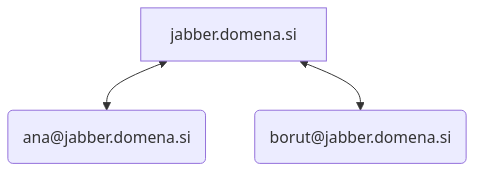
\includegraphics[width=.9\linewidth]{images/local-server.png}
\caption{Komunikacija med uporabniki na istem strežniku}
\end{figure}
\end{frame}

\begin{frame}[label={sec:orgbb2320b}]{Opis specifikacije}
\end{frame}

\begin{frame}[label={sec:orgbd7ec6e}]{Format sporočil}
\end{frame}

\begin{frame}[label={sec:org8b96f50}]{Literatura}
\end{frame}
\end{document}
